\documentclass[12pt]{article}

\usepackage{amssymb, amsmath, lineno, graphicx, float}
\usepackage[margin=1in]{geometry}
\title{The 100-sided Dice Problem}
\author{Arjun Biddanda}
\date{\today}
\pagenumbering{gobble}

\begin{document}
\maketitle
\linenumbers

\subsection*{Problem}

You and I stumble across a 100-sided die in our local game shop. We know we need to have this die — there is no question about it — but we’re not quite sure what to do with it. So we devise a simple game: We keep rolling our new purchase until one roll shows a number smaller than the one before. Suppose I give you a dollar every time you roll. How much money do you expect to win?

\subsection*{Solution}

We will make the assumption that each dice roll is independent. Our real variable of interest is the number of dice rolls that we are able to roll. It might be easier to think of this in terms of an $n$-sided die. We can then have the following setup:

\begin{align*}
Z &\sim \text{\# times dice rolled}\\
\mathbb{E}[Z] &= 1 + \sum^n_{i=2} \mathbb{P}(X_1 ... > X_{i-1} > X_i)\\
\end{align*}

The critical question to ask is if we throw the dice $Z = z$ times, what is the probability that all of the outcomes ($X$) will be descending in order:

$$ \mathbb{P}(X_z < X_{z-1} < ... < X_1) = \frac{\binom{n}{z}}{n^z}$$

Therefore we can use this fact to compute the expected value of $Z$ where we get a $\$c$ payment on each roll:

\begin{align*}
\mathbb{E}[Z] &= \sum^n_{z = 1} c \cdot \frac{\binom{n}{z}}{n^z}\\
&= c \sum^n_{z = 1} \frac{(n-1)!}{z!(n-z)!n^{z-1}}\\
&= c \sum^n_{z = 1} \frac{(n-1)_{(z+1)}}{z!n^{z-1}}\\
\end{align*}


We can then plot the expectation across a number of different sizes of dice $n$:


\begin{figure}[H]
	\begin{center}
		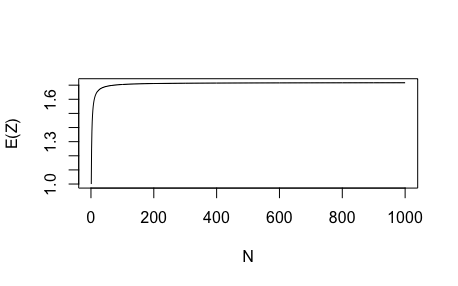
\includegraphics[scale=0.90]{../plots/dice}
		\caption{Expectation of Winnings according to the size of the Die}
	\end{center}
\end{figure}






\end{document}
